\documentclass[letterpaper, 10 pt]{article} 

\usepackage{amsmath}
\usepackage{textcomp}
\usepackage{graphicx}
\usepackage[font=footnotesize]{subcaption}
\usepackage[font=footnotesize]{caption}
\usepackage{hyperref}
\usepackage{amssymb}
\usepackage{booktabs}
\usepackage[normalem]{ulem}
\usepackage{verbatim}
\usepackage[export]{adjustbox}
\usepackage{amsmath}
\usepackage{url}
\usepackage{siunitx}
\usepackage[utf8]{inputenc}
\usepackage[TS1,T1]{fontenc}
\usepackage{array, booktabs}
\usepackage{caption}
\usepackage[cal=cm]{mathalfa}
\usepackage{multirow}

% Labels in IEEE format
\newcommand{\eref}[1]{(\ref{#1})} % Equation
\newcommand{\sref}[1]{Sec.~\ref{#1}} % Section
\newcommand{\figref}[1]{Fig.~\ref{#1}} % Figure
\newcommand{\tref}[1]{Table~\ref{#1}} %Table
\newcommand{\aref}[1]{Algorithm~\ref{#1}} %Algorithm
\renewcommand*\rmdefault{ppl}
\setlength{\textfloatsep}{5pt}

\usepackage{ifthen}
\usepackage[usenames,dvipsnames,table]{xcolor}
\newboolean{include-notes}
\setboolean{include-notes}{true} 
% http://en.wikibooks.org/wiki/LaTeX/Colors
\newcommand{\rhnote}[1]{\ifthenelse{\boolean{include-notes}}%
 {\textcolor{blue}{\textbf{RH: #1}}}{}}
\newcommand{\sanote}[1]{\ifthenelse{\boolean{include-notes}}%
 {\textcolor{green}{\textbf{SAN: #1}}}{}}


\begin{document}

% paper title
\title{6.857 Final Project: Milestone 4}
\author{Sebastiani Aguirre Navarro and Rachel Holladay}
\maketitle

\section{Initial Results}
\label{sec:results}
% “For milestone 4: Get an initial version of your system running end-to-end and produce initial results”

Our goal is to use machine learning techniques to predict the probability of successfully grasping an unknown object with a robotic arm.
We were forced to change our data set, for reasons explained in depth in \sref{sec:risk}, to the Dexerity Network (DexNet) 2.0 data set~\cite{mahler2017dex}.
The data set has 6.7 million synthetic point clouds with parallel-jaw grasps (a common robot hand type of two parallel fingers) and analytical grasp metrics. 

The data set covers 1,5000 3D object models used in DexNet 1.0~\cite{mahler2016dex} that are collected from a variety of other data bases and standardized with respect to position. 
Each object is paired with 2.5D point clouds, which are referred to as depth images, which are rendered with a variety of object and camera poses, where the camera intrinsics are known and used to center the depth image in a standardized fashion.
Each image is a black and white 32 by 32 pixel matrix. 
The parallel jaw grasps were sampled with rejection sampling for antipodal point pairs. 
The grasps are represented by a 7 dimensional vector specifying details of the grasp center, angle, object center and gripper width. 
Together the depth image and grasp vector compose our input. 

Our label is given by the robust epsilon quality grasp metric (defined in~\cite{seita2016large}), which is thresholded by the value 0.002 to create binary labels.

For our initial results we sampled 10,000 data points from the 6.7 millon. 
\rhnote{Describe network and initial results} \figref{fig:accuracy}

\begin{figure}[t!]
    \centering
        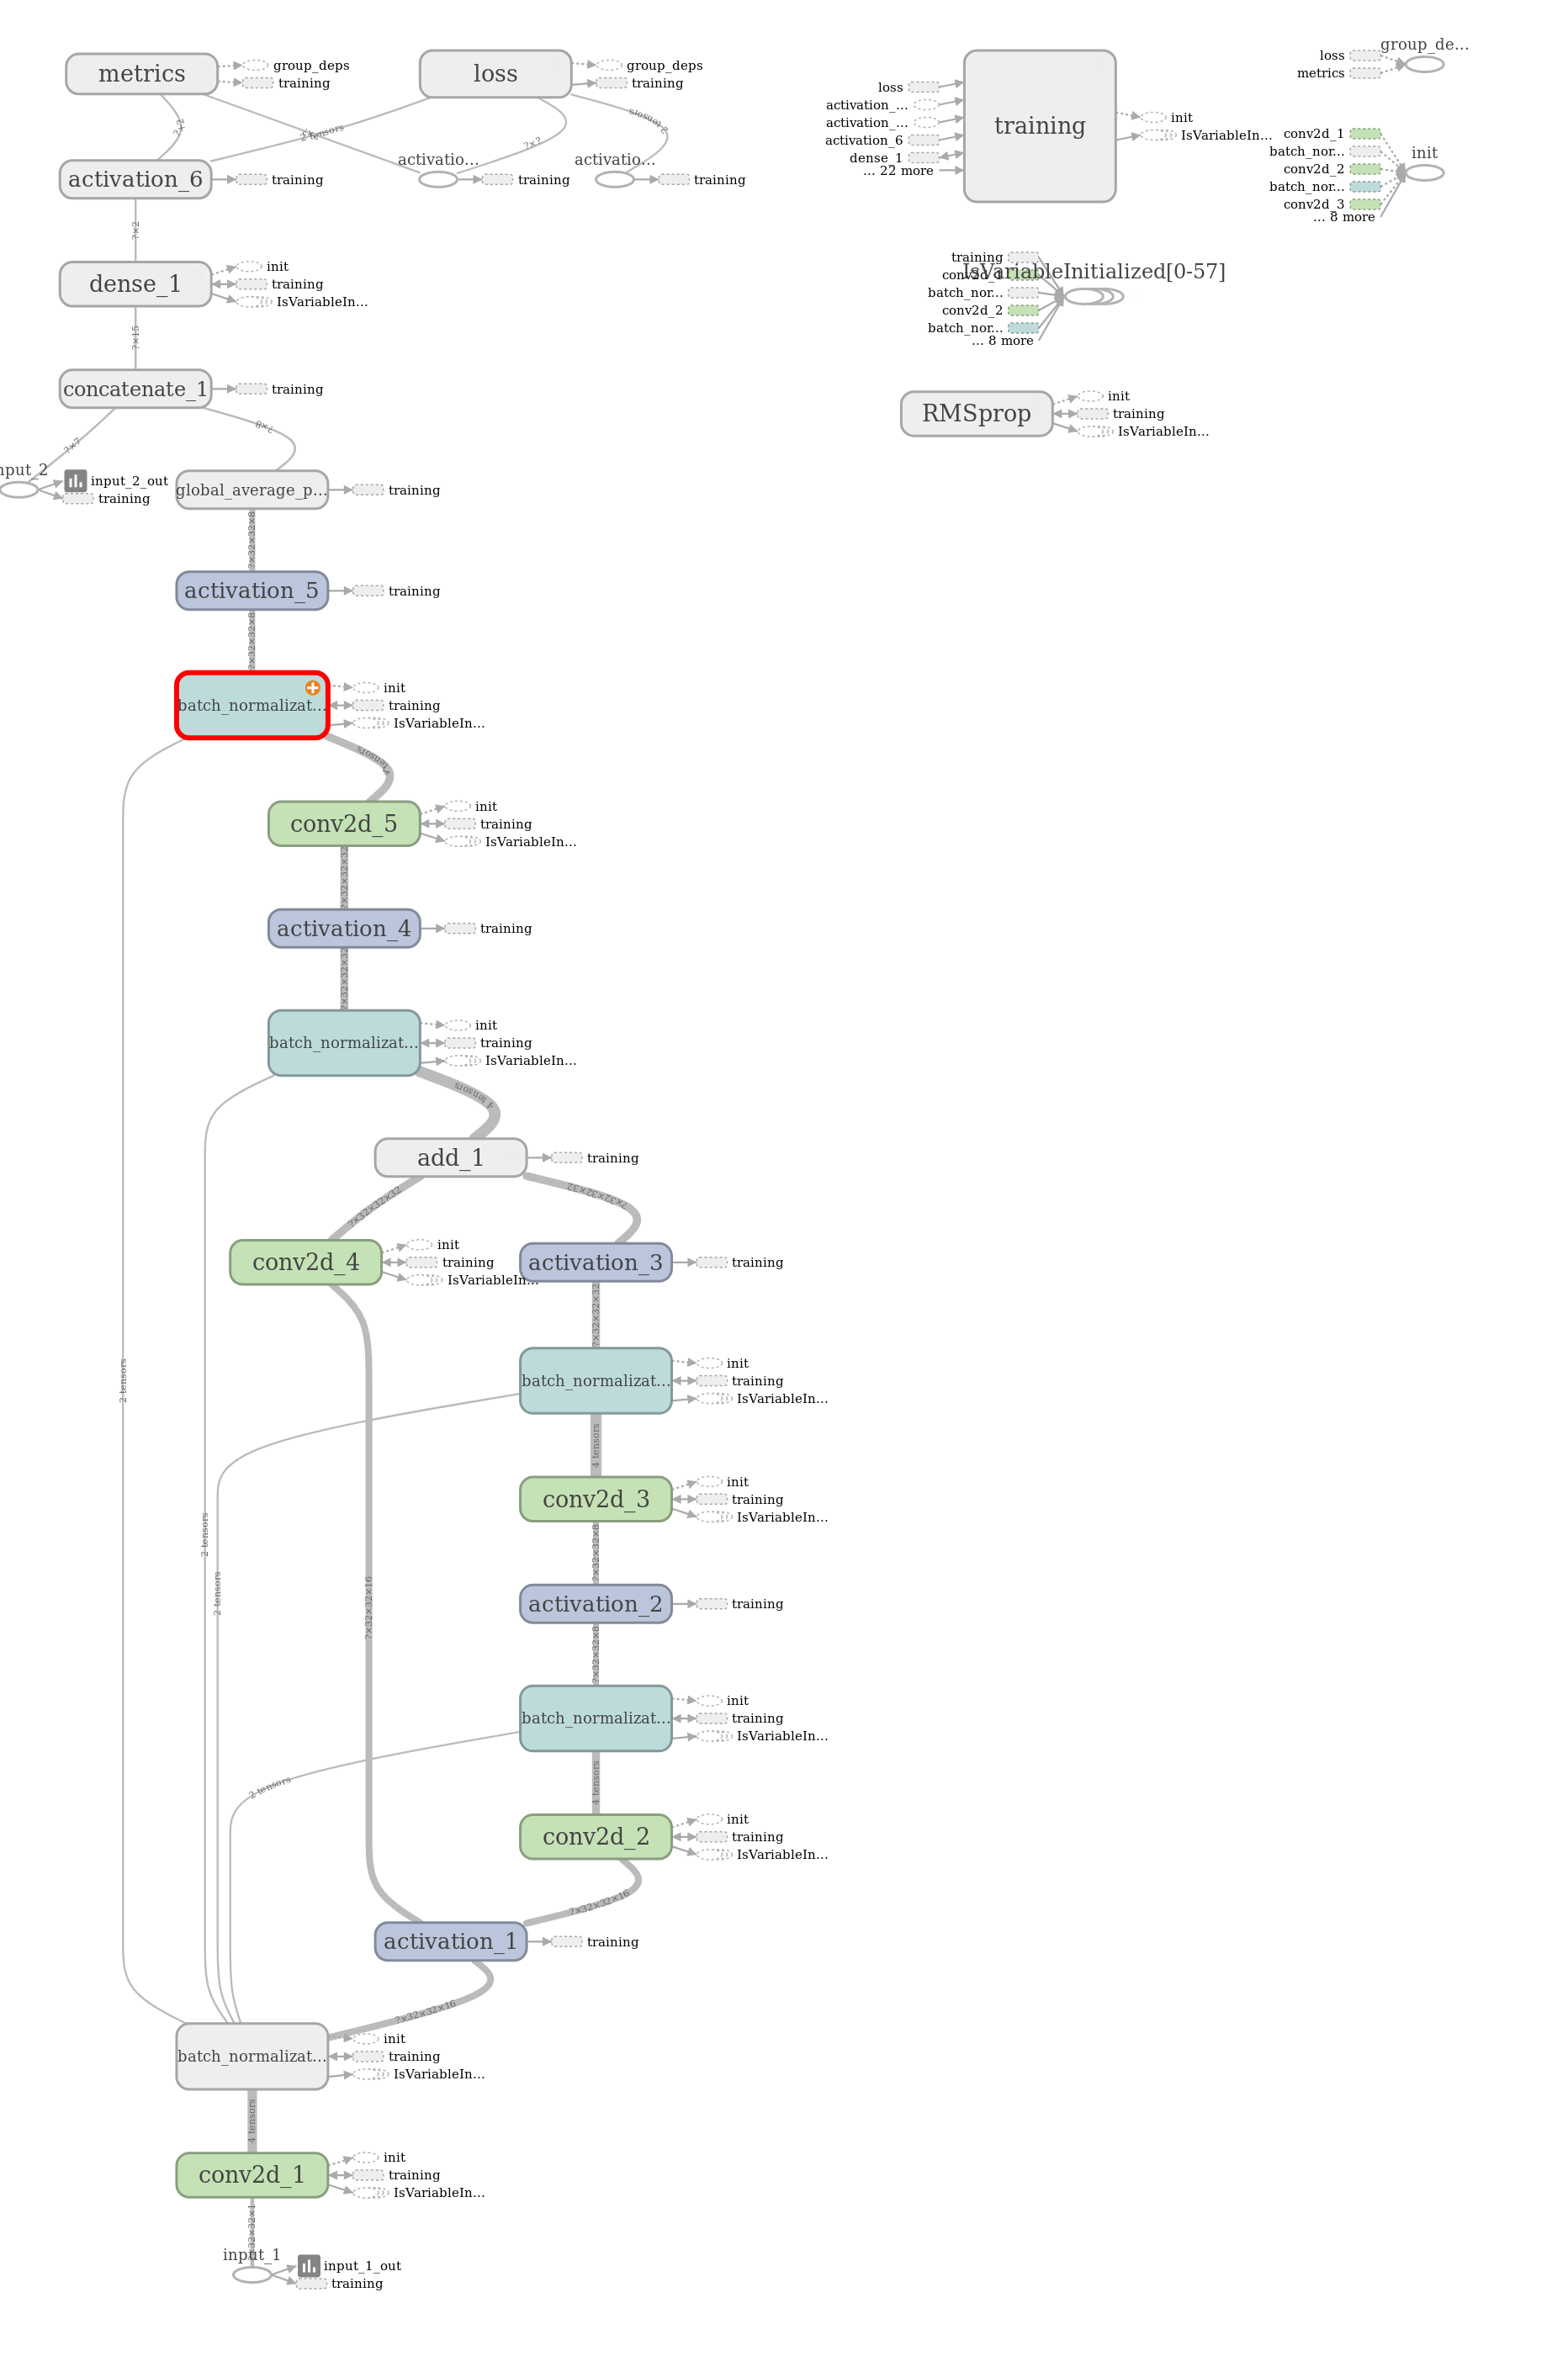
\includegraphics[width=0.5\columnwidth]{figs/dex_resnet.png}
    \caption{Network Structure} \label{fig:network}
\end{figure}

\begin{figure*}[t!]
    \begin{subfigure}[t]{0.49\textwidth}
        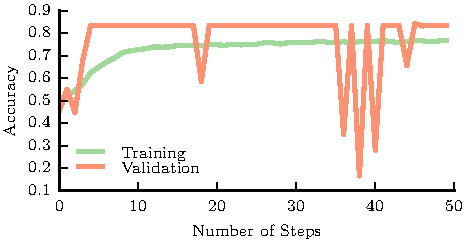
\includegraphics[width=0.99\columnwidth]{figs/accuracy.pdf}
        \caption{Accuracy} \label{fig:accuracy}
        \end{subfigure}
    \begin{subfigure}[t]{0.49\textwidth}
        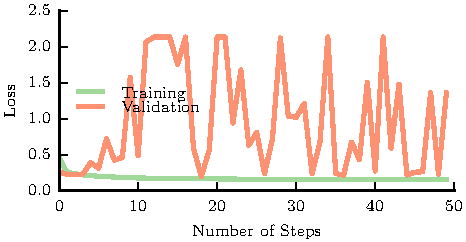
\includegraphics[width=0.99\columnwidth]{figs/loss.pdf}
        \caption{Loss} \label{fig:loss}
    \end{subfigure}
\caption{Insert Caption} \label{fig:results}
\end{figure*}


\begin{comment}
Given our labeled data, when can then turn to our learning algorithms. 
We will use Tensorflow and Keras to implement our learning algorithms. Keras specifically containes predefined many of the common layers used in deep neural networks.
This will prove useful to run initial prototypes that build upon these common layers. Eventually, we will have to tweak the layers or add layers that are not predefined in Keras.
This is where we will turn to Tensorflow. While Tensorflow already has many basic predefined layers, prototyping in it can be tedious. However Tensorflow provides the fundamental tools for defining custom operations and layers.
There is also an existing ``Model Zoo'' for Keras and Tensorflow. Since many of the proposed architectures have been already trained with the purpose of detecting or classifying objects, one strategy is to properly modify the input layers and
perform Transfer Learning to see if we can reduce the training time significantly in our grasper network when tuning it on the RGBD data. We will also write from scratch several prototypes that apply the concepts of ResNet, Network in Network
and Inception so that we can compare it to other transfered off the shelf models. 
\end{comment}

\section{Risk Mitigation}
\label{sec:risk}
One of the risks we had mentioned in a previous milestone relating to data access unfortunately became realized. 
Early in our project we mentioned two possible datasets, the BigBird data set~\cite{singh2014bigbird} and the DexNet data set~\cite{mahler2017dex}.
We elected to use the BigBird data set in conjunction with the grasp generation and labeling process package "Grasp Pose Generator (GPG)" from~\cite{pas2017grasp}.
In attempting to create our training data, we realized that GPG did not directly use the data in the BigBird set and instead first performed a transformation that editted the depth files and generated surface normals. 
We were unable to find the opensource component that performed this transformation and the author of the report (at the time of this writing) has not replied to our request. 

Therefore, we have switched to using the DexNet 2.0 data set, whose data is described in further detail in \sref{sec:results}. 
If we are able to use the BigBird data set, we will consider using it in conjunction or as a comparison. 

\section{Division of Labor}

Rachel generated the training data from the DexNet data sets and set of the labeling mechanism. 
Sebastiani will set up an environment in a cloud provider with GPUs and start coding the Network In Network and Inception based models in Keras/Tensorflow and transfer learn layers of a pretrained YOLO onto our problem space.  \rhnote{This is what we had written last time. Is it still correct?}

{\footnotesize
    \bibliographystyle{ieeetr}
\bibliography{../references}}

\end{document}
